% Gemini theme
% https://github.com/anishathalye/gemini

\documentclass[
    final,
    ]{beamer}

% ====================
% Packages
% ====================

\usepackage[T1]{fontenc}
\usepackage{lmodern}
\usepackage[size=custom, width=120, height=67.5, scale=0.99]{beamerposter}
\usetheme{gemini}
\usecolortheme{gammapy}
\usepackage{graphicx}
\usepackage{booktabs}
\usepackage{tikz}
\usepackage{pgfplots}
\usepackage{fontawesome5}
\usepackage{orcidlink}
\setbeamerfont{caption name}{series=\bfseries}
\setbeamerfont{footline}{size=\fontsize{32}{11}\selectfont}

% ====================
% Lengths
% ====================

% If you have N columns, choose \sepwidth and \colwidth such that
% (N+1)*\sepwidth + N*\colwidth = \paperwidth
\newlength{\sepwidth}
\newlength{\colwidth}
\setlength{\sepwidth}{0.025\paperwidth}
\setlength{\colwidth}{0.3\paperwidth}

\newcommand{\separatorcolumn}{\begin{column}{\sepwidth}\end{column}}
\newcommand{\coloredhref}[3][blue]{\href{#2}{\color{#1}{#3}}}%
\newcommand*{\mathscale}[2][4]{\scalebox{#1}{\ensuremath{#2}}}%
\newcommand{\gammapysymbol}{\mathscale[1.5]{\raisebox{6pt}{\gamma} \pi}}

% ====================
% Title
% ====================

\title{Gammapy: a Python Package for Gamma-Ray Astronomy}

\author{
    \textbf{Axel Donath} \orcidlink{0000-0003-4568-7005} \inst{1} \and
    \textbf{R\'{e}gis Terrier} \orcidlink{0000-0002-8219-4667} \inst{2} \and
    Jos\'{e} Enrique~Ruiz \orcidlink{0000-0003-3274-4445} \inst{5} \and
    Quentin Remy \inst{1} \and
    Atreyee Sinha \orcidlink{0000-0002-9238-7163} \inst{3} \and
    Fabio~Pintore \inst{7} \and
    Laura~Olivera-Nieto  \orcidlink{0000-0002-9105-0518} \inst{1} \and
    Luca Giunti \inst{4} \and
    Fabio~Acero \orcidlink{0000-0002-6606-2816} \inst{6} \and
    Cosimo~Nigro~\orcidlink{0000-0001-8375-1907}~\inst{8} \and
    Alexis de Almeida Coutinho~\inst{10} \and
    Bruno~Khelifi~\orcidlink{0000-0001-6876-5577} \inst{2} \and
    Maximilian N\"{o}the \inst{9} \and
    Jalel Eddine Hajlaoui \inst{2} \and
    for the Gammapy development team
  }

\institute[shortinst]{
    \inst{1} MPIK Heidelberg \samelineand
    \inst{2} APC Paris \samelineand
    \inst{3} LUPM Montpellier \samelineand
    \inst{4} CEA Paris \samelineand
    \inst{5} IAA-CSIC Granada \samelineand
    \inst{6} AIM/CEA Saclay-CNRS \samelineand
    \inst{7} INAF-IASF Palermo \samelineand
    \inst{8} IFAE Barcelona \samelineand
    \inst{9} TU Dortmund \samelineand
    \inst{10} Universidade de S\~{a}o Paulo
    }

% ====================
% Footer (optional)
% ====================

\footercontent{
  \href{https://gammapy.org}{\gammapysymbol~~Webpage} \hfill
  \href{https://docs.gammapy.org}{\gammapysymbol~~Documentation} \hfill
  \href{https://github.com/gammapy/gammapy/}{\faGithub~~Github}  \hfill
  \href{https://twitter.com/gammapyst}{\faTwitter~~Twitter}  \hfill
  \href{https://gammapy.slack.com/}{\faSlack~~Slack}  \hfill
  \href{https://gammapy.org/gammapy_song.mp3}{\faMusic~~Song}  \hfill
  \href{https://indico.desy.de/event/27991/contributions/102086/}{ICRC 2021, Berlin}
  }
% (can be left out to remove footer)

% ====================
% Logo (optional)
% ====================

% use this to include logos on the left and/or right side of the header:
\logoright{
\includegraphics[height=7cm]{figures/gammapy_logo_white.pdf}}
% \logoleft{\includegraphics[height=7cm]{logo2.pdf}}

% ====================
% Body
% ====================

\begin{document}

\begin{frame}[t, fragile]
\begin{columns}[t]
\separatorcolumn

\begin{column}{\colwidth}

  \begin{block}{Abstract}

\heading{Overview}
Gammapy is a community-developed, open source Python package for gamma-ray astronomy, 
which is built on the scientific Python ecosystem including \coloredhref[pink]{https://numpy.org}{Numpy},
\coloredhref[pink]{https://scipy.org}{Scipy} and \coloredhref[pink]{https://astropy.org}{Astropy}.
It provides methods for the analysis of gamma-ray data of many existing instruments including
imaging atmospheric Cherenkov telescopes, such as \coloredhref[pink]{https://www.mpi-hd.mpg.de/hfm/HESS/}{HESS}, \coloredhref[pink]{https://magic.mpp.mpg.de}{MAGIC} and \coloredhref[pink]{https://veritas.sao.arizona.edu}{VERITAS}, water Cherenkov observatories such as \coloredhref[pink]{https://www.hawc-observatory.org}{HAWC}, as well as space-based observatories such as \coloredhref[pink]{https://fermi.gsfc.nasa.gov}{Fermi-LAT}. Gammapy has also recently been selected as the package of choice for the \coloredhref[pink]{https://www.cta-observatory.org/ctao-adopts-the-gammapy-software-package-for-science-analysis/}{CTA Science Tools}.


\heading{Main Features}
Starting from event lists and a description of the specific instrument response functions (IRF)
stored in an \coloredhref[pink]{https://gamma-astro-data-formats.readthedocs.io/en/latest/}{open FITS based data format}, Gammapy implements the reduction of the input data
and instrument response to binned data structures. 
Thereby it handles the dependency of the data and IRFs with energy as well as position on the sky.
It offers a variety of background estimation methods for spectral, spatial and spectro-morphological 
analysis. Counts, background and IRFs data are bundled in datasets and can be serialised, rebinned
and stacked.

Gammapy allows for reduction and subsequent modelling of binned data using Poisson maximum likelihood fitting.
It comes with \coloredhref[pink]{https://docs.gammapy.org/0.18.2/modeling/gallery/index.html\#model-gallery}{built-in spectral, spatial and temporal models} as well as support for custom user models,
to model e.g. \coloredhref[pink]{https://docs.gammapy.org/0.18.2/tutorials/models.html\#Models-with-Energy-dependent-morphology}{energy-dependent morphology} of gamma-ray sources. Multiple datasets
can be combined in a joint-likelihood approach to either handle time-dependent IRFs, different classes
of events or combination of data from multiple instruments. Gammapy also implements
methods to estimate flux points, including likelihood profiles per energy bin, light curves as well as
flux and significance maps in energy bins.

  \end{block}

  \begin{block}{Analysis Example I}
    \begin{figure}
      \centering
      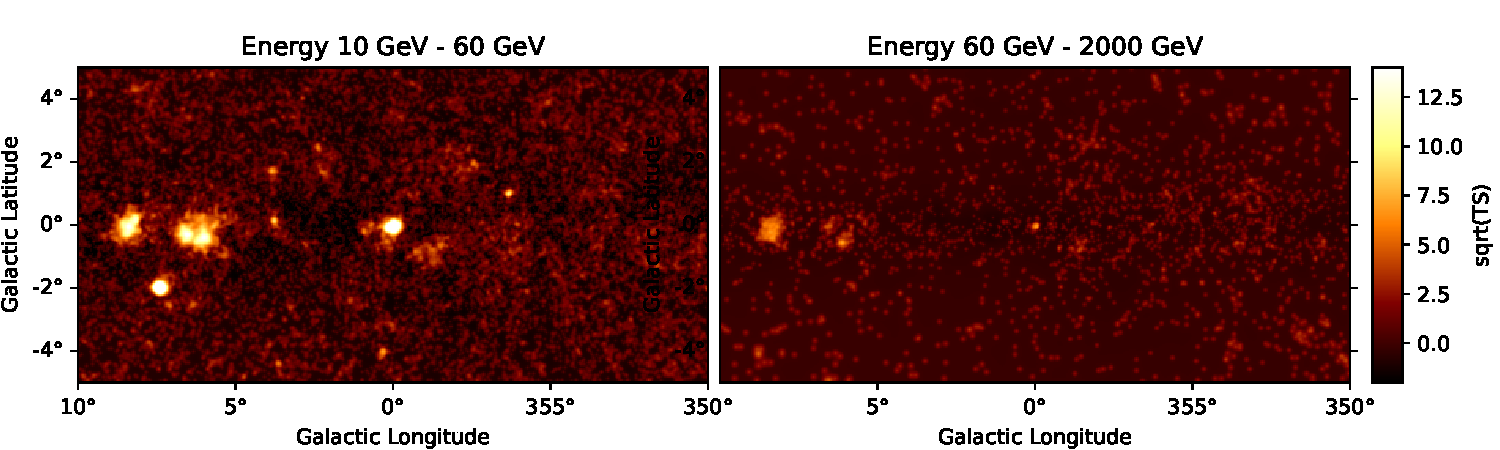
\includegraphics[width=\textwidth]{figures/fermi-gc-sqrt-ts.pdf}
      \caption{TS-maps in two energy bands computed for \coloredhref[pink]{https://fermi.gsfc.nasa.gov}{Fermi-LAT} (3FHL) data in the Galactic Center region. The TS-maps are computed assuming a point-like source morphology and a power-law shaped spectral model with spectral index of $\Gamma = 2$. The example is adapted from the \coloredhref[pink]{https://docs.gammapy.org/0.18.2/tutorials/detect.html}{source detection tutorial}.}
    \end{figure}
 
  \end{block}

\end{column}

\separatorcolumn

\begin{column}{\colwidth}

  \begin{alertblock}{Install Gammapy}

    The recommended way to install Gammapy is to \coloredhref[pink]{https://www.anaconda.com/products/individual}{download the Anaconda Python distribution} and then create a new virtual environment
    from the dedicated conda environment file:
%
    \begin{verbatim}
$ curl -O https://gammapy.org/download/install/gammapy-0.18.2-environment.yml
$ conda env create -f gammapy-0.18.2-environment.yml
$ conda activate gammapy-0.18.2
    \end{verbatim}
%
    \vspace{-24pt} 
    For more detailed instructions and other ways to install Gammapy see \coloredhref[pink]{https://docs.gammapy.org/0.18.2/install/index.html}{installation instructions}.
  \end{alertblock}

  \begin{block}{Gammapy Package and API}
  Gammapy is structured into sub-packages corresponding to the different data levels and transitions between them. Gammapy can be typically \coloredhref[pink]{https://docs.gammapy.org/0.18.2/tutorials/analysis_2.html}{used as a standard Python library} by importing the functionality from the sub-packages, but there is also a configuration file based \coloredhref[pink]{https://docs.gammapy.org/0.18.2/tutorials/analysis_1.html}{high level analysis API}.
    \begin{figure}
      \centering
      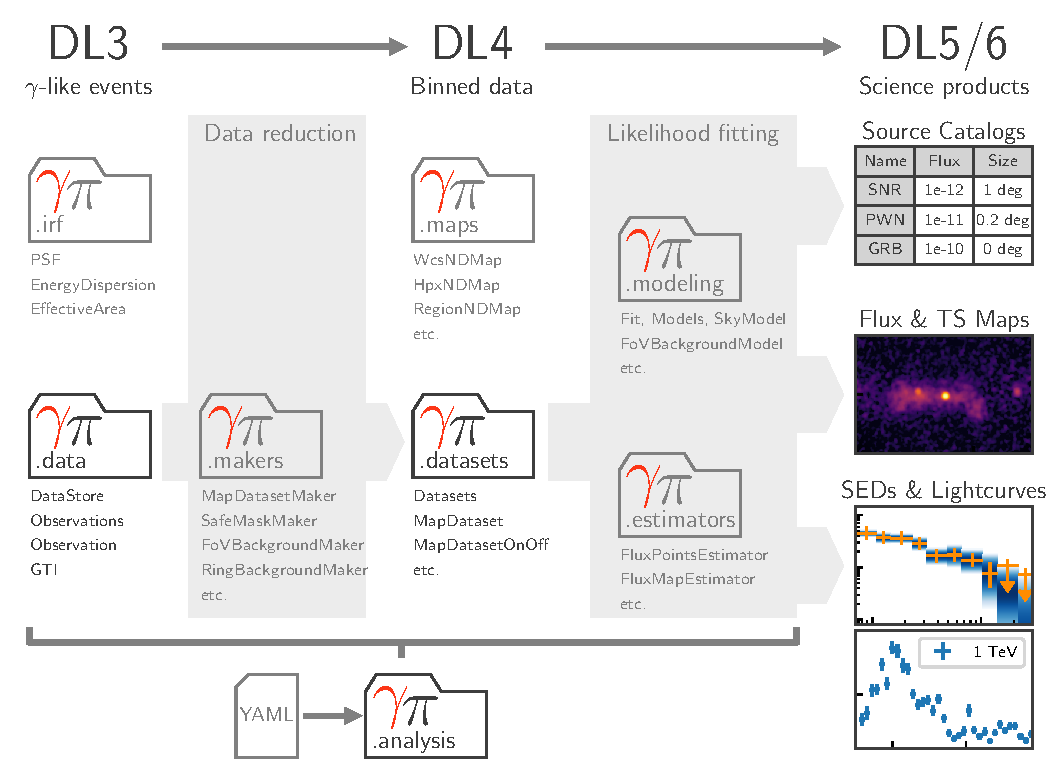
\includegraphics[width=\textwidth]{figures/data-flow-gammapy.pdf}
      \caption{Data flow and sub-package structure of Gammapy. The folder icons represent the corresponding sub-packages. The direction of the the data flow is illustrated with shaded arrows. The top section shows the data levels as defined by \coloredhref[pink]{https://www.cta-observatory.org}{CTA}.}
    \end{figure}

  %Gammapy is structured into sub-packages.

  \end{block}
\end{column}

\separatorcolumn

\begin{column}{\colwidth}

  \begin{block}{Analysis Example II}

    \begin{figure}
      \centering
      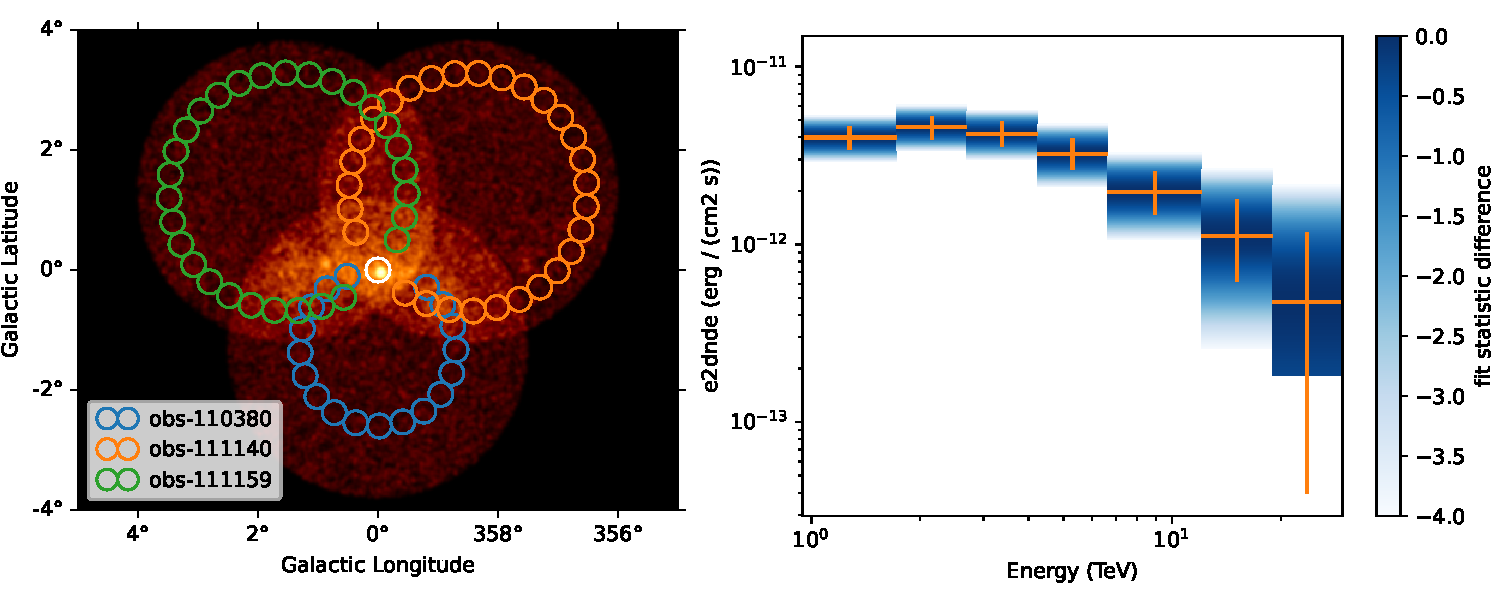
\includegraphics[width=\textwidth]{figures/cta-gc-image-spectrum.pdf}
      \caption{Spectral analysis of multiple simulated \coloredhref[pink]{https://www.cta-observatory.org}{CTA} observations in the Galactic Center region. The left image illustrates the reflected regions used for the  background estimation of the spectrum, the right image shows the estimated flux points with the
      corresponding likelihood profiles. The example is adapted from the \coloredhref[pink]{https://docs.gammapy.org/0.18.2/tutorials/cta_data_analysis.html}{cta data analysis tutorial}.}
    \end{figure}
  \end{block}
  \vspace{-36pt} 
  \begin{block}{Science Validation and Analyses using Gammapy}
  Gammapy is already used for many interesting analysis of real and simulated data of many different instruments, such as \coloredhref[pink]{https://www.mpi-hd.mpg.de/hfm/HESS/}{HESS}, \coloredhref[pink]{https://www.hawc-observatory.org}{HAWC} and \coloredhref[pink]{https://www.cta-observatory.org}{CTA}. The following list highlights a few selected studies presented at this ICRC 2021:

  \begin{itemize}
    \item \coloredhref[pink]{https://indico.desy.de/event/27991/contributions/101917/}{Survey of the Galactic Plane with the Cherenkov Telescope Array}
    \item \coloredhref[pink]{https://indico.desy.de/event/27991/contributions/101910/}{Revisiting the PeVatron candidate MGRO J1908+063 with an updated H.E.S.S. analysis}
    \item \coloredhref[pink]{https://indico.desy.de/event/27991/contributions/101942/}{Discovery of 100 TeV gamma-rays from HESS J1702-420: a new PeVatron candidate}
    \item \coloredhref[pink]{https://indico.desy.de/event/27991/contributions/101938/}{Search for enhanced TeV gamma ray emission from Giant Molecular Clouds using H.E.S.S.}
    \item \coloredhref[pink]{https://indico.desy.de/event/27991/contributions/101937/}{The young massive stellar cluster Westerlund 1 in gamma rays as seen with H.E.S.S.}
    \item \coloredhref[pink]{https://indico.desy.de/event/27991/contributions/102013/}{Standardized formats for gamma-ray analysis applied to HAWC observatory data}
  \end{itemize}

Gammapy has been validated using \coloredhref[pink]{https://www.mpi-hd.mpg.de/hfm/HESS/pages/dl3-dr1/}{public H.E.S.S. data} in \cite{Mohrmann2019} and has been used for an open and reproducible multi-instrument analysis of the Crab Nebula in \cite{Nigro2019}. The validation of reference results and performance bechmarks are executed and documented continuously in the corresponding \coloredhref[pink]{https://github.com/gammapy/gammapy-benchmarks}{Gammapy benchmarks repository} on a nightly basis.

  \end{block}

  \begin{block}{References}

    \nocite{*}
    \footnotesize{\bibliographystyle{plainurl}\bibliography{poster}}

  \end{block}

\end{column}

\separatorcolumn
\end{columns}
\end{frame}

\end{document}
